\documentclass[12pt]{article}
\usepackage[margin=1in]{geometry}
\usepackage{graphicx}
\graphicspath{ {./} }


\title{Talkatiel Software Requirements and Planning}
\author{Brendan Byers, Ryan Sisco, Iliana J, Aidan Grimshaw}
\date{\today}

\begin{document}
\begin{center}
      \Large\textbf{Talkatiel Design Implementation System}\\
      \large\textit{Brendan Byers, Ryan Sisco, Iliana J, Aidan Grimshaw, Yufei Zeng}\\
      \large{byersbr, siscor, javieri, grimshaa, zengyu}\\
   \end{center}

\tableofcontents

\section{UML Class Diagram}
\begin{center}
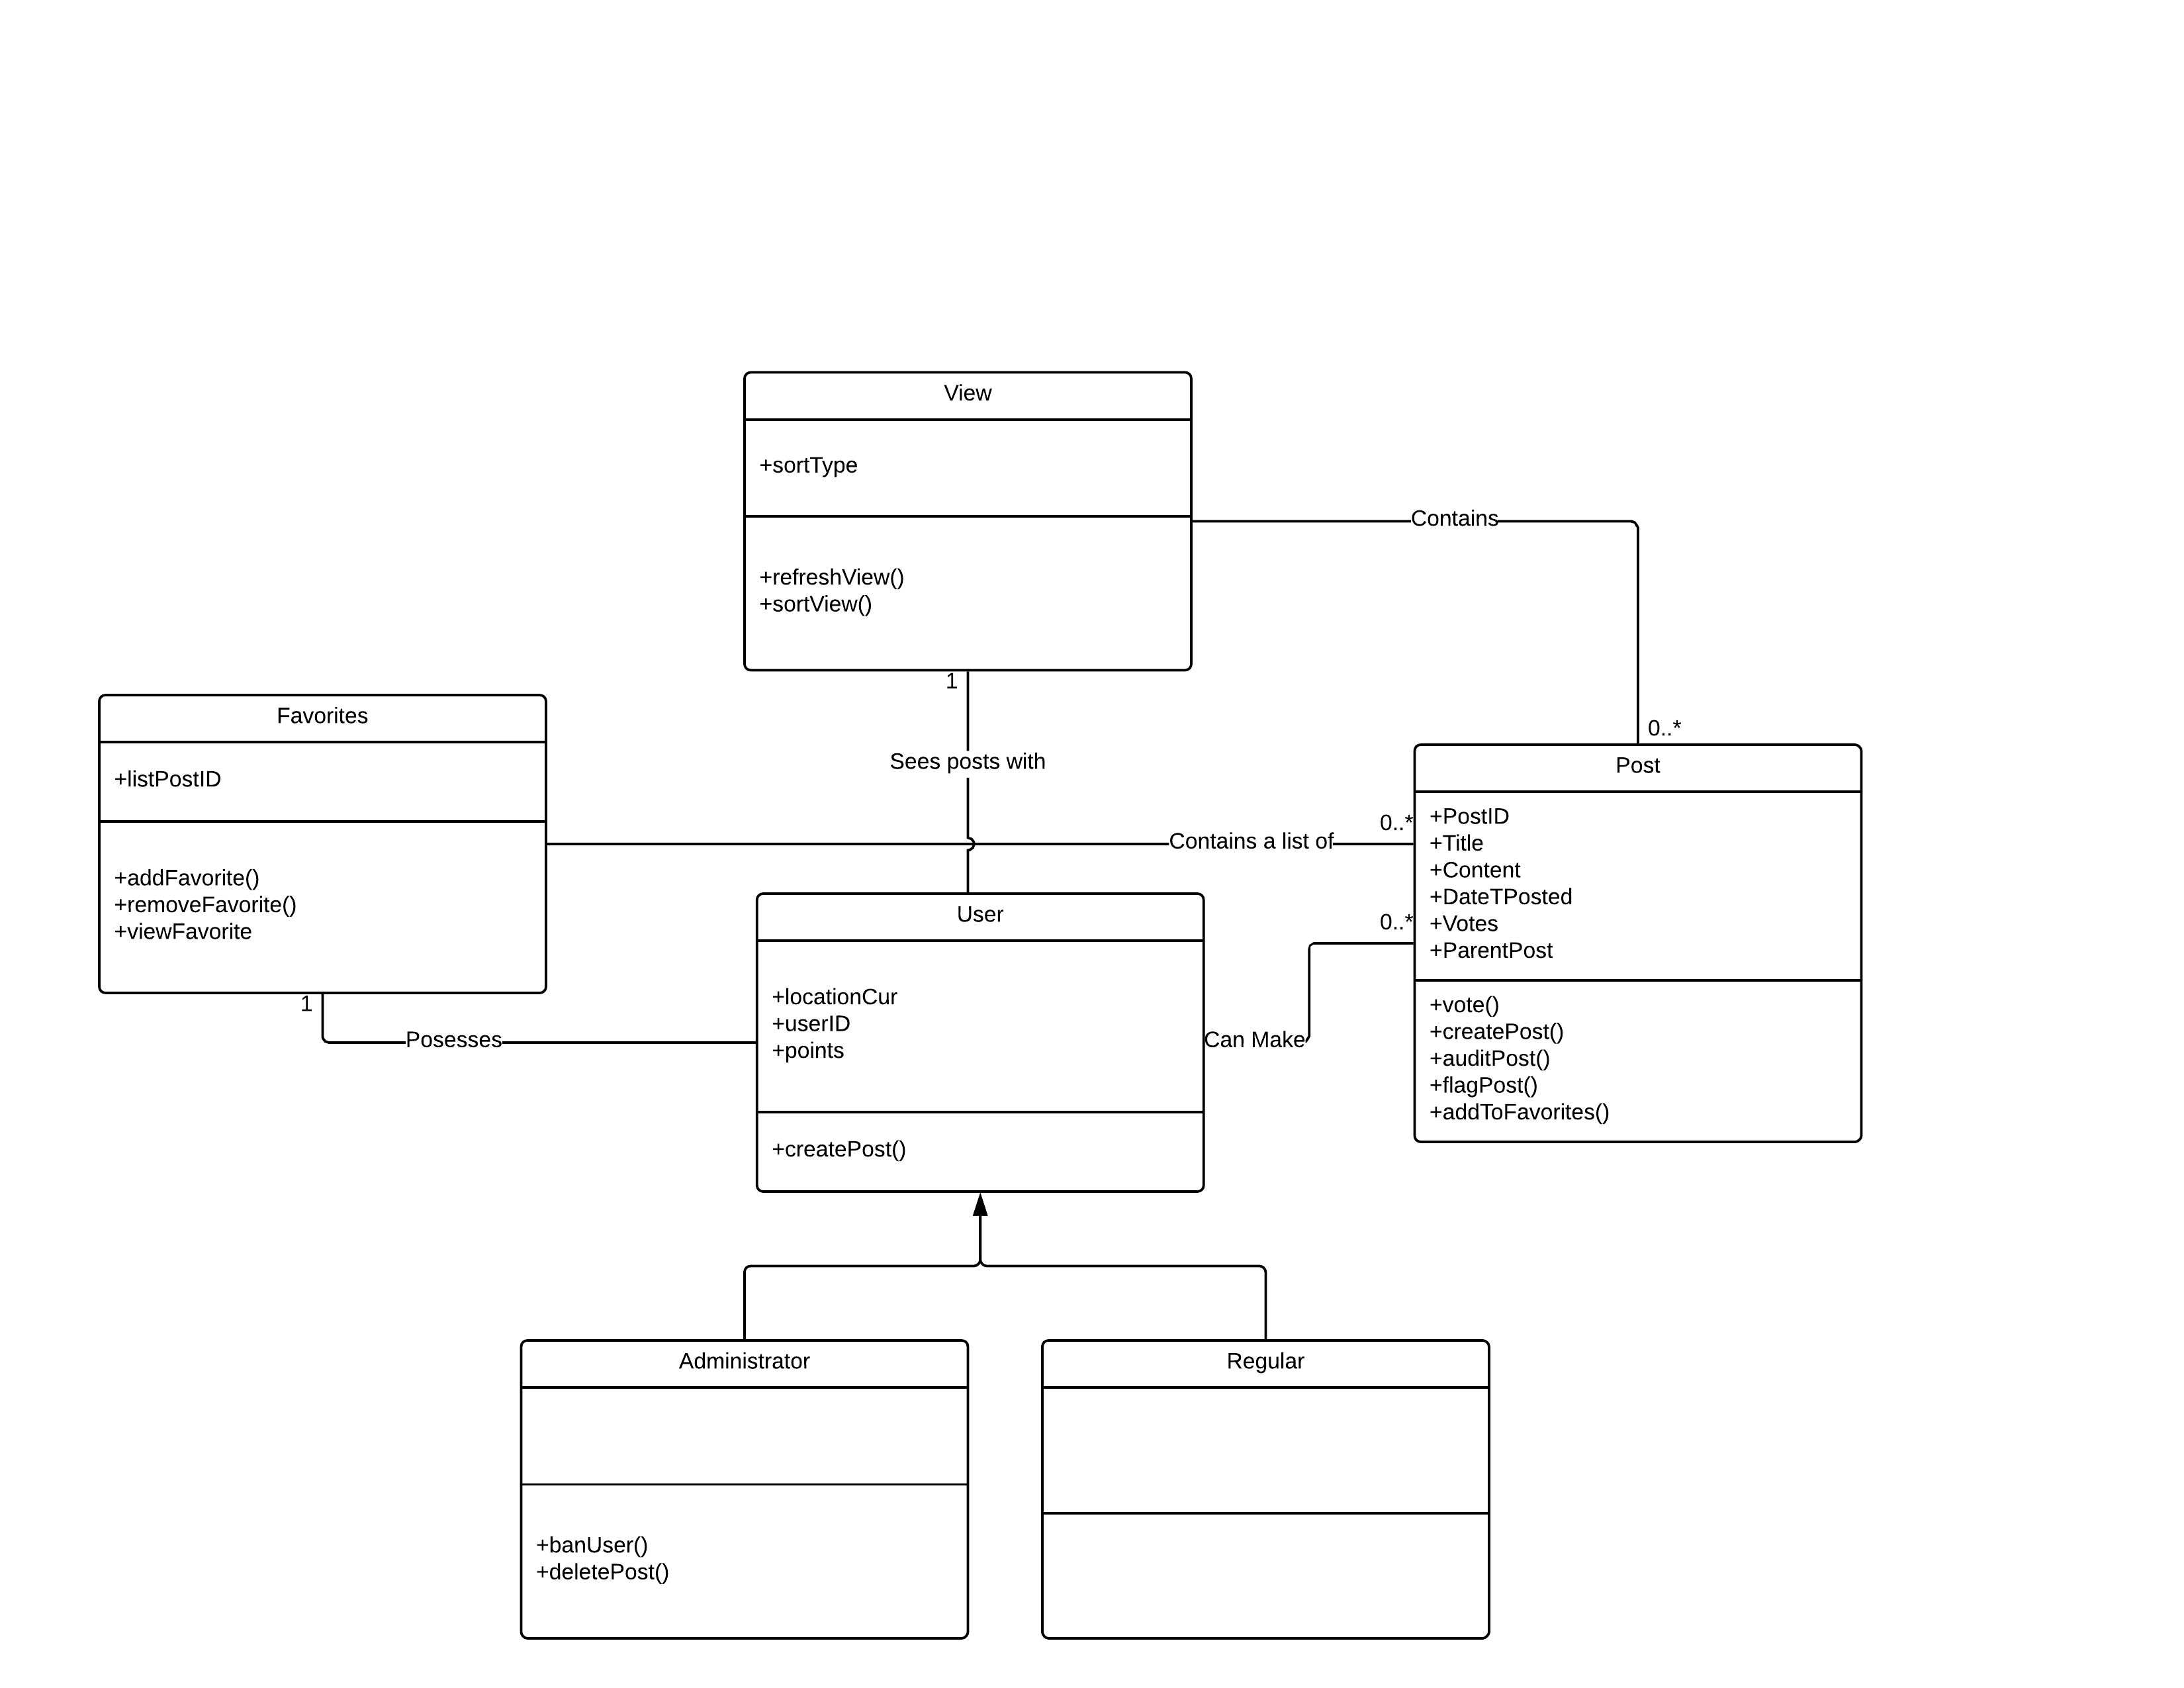
\includegraphics[scale=0.25]{img/uml/ClassDiagram}\linebreak
\textbf{Class Diagram}
  \end{center}

\section{Packages}

\section{Design Patterns}

\section{Exceptions & Handling}

\section{Meeting report}
\subsection{Progress Made this Week}

This week we worked on getting the different parts of assignment 4 together and assembling the presentation.  We worked on solidifying the design patterns and strategy to make them clearer for both us the programmers and the customer.  We started thinking about direct coding decisions when it came to handling different types of exceptions that may come up.  Additionally we compacted everything into a slide show and practiced presenting in preparation for either tuesday or thursday.

\subsection{Plans for Next Week}

Next we will start nailing down individual user stories for different actions that a user can do.  This will include making a post, voting on a post, fetching a posts or moderating posts.  This will enable us to better plan how to implement these features.  We will also start preparing to program by setting up the toolchain and agreeing on a coding style.

\subsection{Team Member Contributions}

UML Class Diagram - Brendan Byers

Packages - Iliana Javier

Design Patterns - Aiden Grimshaw

Exceptions & Handling - Yufei Zeng

Meeting Report - Brendan Byers

Requirement and Design Presentation - Ryan Sisco, Aiden Grimshaw, Yufei Zeng, Iliana Javier, Brendan Byers 



\end{document}
